\documentclass[12pt]{article}
\usepackage{amsmath}
\usepackage{amsthm}
\usepackage{amssymb}
\usepackage[left=2cm,top=1cm,right=3cm,bottom=1cm]{geometry}
\usepackage{graphicx}
\usepackage{listings}

\newtheorem{definition}{Definition}
\newtheorem{remark}{Remark}
\newtheorem{theorem}{Theorem}

\begin{document}

\begin{center}\LARGE\bf
    Sorting
\end{center}

\section{Insertion Sort}
Insertion Sort solves the sorting problem:
\newline\textbf{Input}: A sequence of n numbers $\left\langle a_1, a_2, ..., a_n\right\rangle$
\newline\textbf{Output}: A permutation of the input sequence $\left\langle a_1', a_2', ..., a_n' \right\rangle$ where $a_1' \leq  a_2' \leq ... \leq a_n'$.

The numbers to be sorted are known as \textit{keys}. These keys are often associated with other data, which we call \textit{satellite data}. A
key and satellite data form a \textit{record}. When sorting with respect to some key, the satellite data is also sorted so that it stays with the associated
key.

In this text we shall write algorithms in pseudocode. Real implementations in various languages can be found in the same directory as this text.
Some notes regarding conventions. We shall organise compound data into \textit{objects}, composed of \textit{attributes}. Parameters
will be passed \textit{by value}; that is to say, the called procedure receives its own copy of the parameter. Assignments to this parameter
within the called procedure will not be visible to the caller. However, if the parameter is a pointer (for example, pointer $x$ with some
attribute $f$), assignment $x.f = 3$ will be visible to the caller, as will changes to an array, which is passed by a pointer to the first element.

Assume boolean operators are \textit{short circuiting}. That is, for operators \textit{and} and \textit{or}, the left expression will be
evaluated first. The right expression will only be evaluated if the full expression's value isn't determined by
the left expression. For example, if $x \textit{ and } y$, $y$ won't be evaluated if $x$ is false. Similarly, if
$x \textit{ or } y$, $y$ won't be evaluated if $x$ is true.

Insertion sort is an efficient algorithm when sorting a small number of elements.
\begin{lstlisting}
    INSERTION-SORT(A, n)
    for i = 2 to n
        key = A[i]
        // Insert A[i] into the sorted subarray A[1:i-1]
        j = i - 1
        while j > 0 and A[j] > key
            A[j + 1] = A[j]
            j = j - 1
        A[j + 1] = key
\end{lstlisting}

In words, we separate the array of elements into two \textit{subarrays} (that is, contiguous portions of the array), where the
left subarray is sorted and the right may not be. We then iterate through the right array, taking the leftmost element in
the right array (call this the key) and trying to find its correct position by comparing its value with each element in the left
array, from right to left. When there is a value that is less than the key, insert the key to the right of
this value, shifting all the values above this along by one. Repeating this with every element in the right array
will eventually result in a sorted array. See Figure \ref{Figure: insertion sort} for a visual representation.

\begin{figure}[ht]\centering
    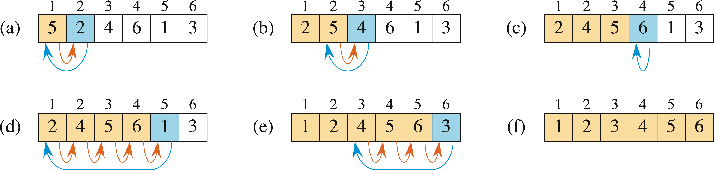
\includegraphics[angle=0]{Figures/insertion-sort.pdf}
    \caption{Visual representation of the insertion sort algorithm.}
    \label{Figure: insertion sort}
\end{figure}

We want to prove that this is a correct algorithm. We can do this by mathematical induction using a \textit{loop invariant}.
A loop invariant is a property of a program that is true before and after each iteration of a loop. Thus, if we can formulate
the desired outcome of our algorithm (in this case, for the array to be sorted) as a loop invariant, then showing that this property
is a valid loop invariant will be equivalent to proving correctness of the algorithm. To show that the loop invariant is corrent we must
show:
\newline \textbf{Initialization}: the property is true before the first iteration of the loop.
\newline \textbf{Maintenance}: if the property is true before a given iteration, it is also true before the next iteration.
\newline \textbf{Termination}: The loop terminates and gives a useful property that helps us to verify that the algorithm is correct.

For example, insertion sort is correct if the final array is sorted. Consider the following loop invariant:
\newline \textit{At the start of each iteration of the for loop, the subarray \texttt{A[1:i-1]} consists of the elements originally in \texttt{A[1:i-1]},
but in correct sorted order}.

To prove correctness of insertion sort, we prove the loop invariant always holds by induction:
\newline \textbf{Initialization}: Before the first loop iteration\footnote{In a \texttt{for} loop, this is between the counter initialization \texttt{int i = 2} and the condition
i $\leq$ n assuming a C \texttt{for} loop: \texttt{for (int i = 2; i $\leq$ n; i++)}.}, i = 2 so the left
subarray is just \texttt{A[1:i-1]} = \texttt{A[1]}, which clearly contains the original element and is sorted.
\newline \textbf{Maintenance}: Formally, we should check the while loop with a loop invariant. Informally, each interation
moves the values by one until \texttt{A[i]} is placed in the correct position. This implies that \texttt{A[1:i]}
is still sorted and contains the same elements. Thus, \textit{incrementing} i preserves this.
\newline \textbf{Termination}: To conclude our proof, we want to take the condition that terminates the loop and sub
it into the original formulation of the loop invariant above. This should give us a statement that proves the correctness of the
algorithm. The loop stops where $i > n$, or equivalently, $i = n + 1$. Subbing this in gives the following statement:
\textit{The subarray A[1:n] consists of elements originally in A[1:n] but in sorted order}. This is exactly our goal (that is, array A
has been sorted) and so this proves correctness by induction.

\textit{Linear search} solves the following \textit{searching problem}:
\newline \textbf{Input:} A sequence of $n$ numbers $\left\langle a_1, a_2, ..., a_n\right\rangle$ stored in array
A[1:n] and a value $x$.
\newline \textbf{Output:} An index $i$ such that $x$ equals A[i] or the special value \texttt{NIL} if x does not appear
in A.

Linear search scans the array from beginning to end, looking for $x$:
\begin{lstlisting}
    LINEAR-SEARCH(A, n, x)
    for i in 1 to n
        if A[i] = x
            return i
    return NIL
\end{lstlisting}

Prove its correctness with the following loop invariant: \textit{At the start of each iteration, the
subarray \texttt{A[1:i-1]} contains only elements not equal to x}. This is valid as the loop terminates when
returning either $i$ or \texttt{NIL}.

\section{Analysis of Algorithms}
Analysing an algorithm has come to mean predicting the resources that it requires, most commonly time (and memory). In the \textit{random-access
machine} (RAM) model of computation, each instruction or data access takes a constant amount of time, and
no operations occur concurrently. Note that we can't assume that every instruction takes constant time as this
would lead to an unrealistic and unhelpful model. For example, an instruction that sorts in a single instruction,
would be assumed to take constant time in the RAM model, which is unrealistic. Thus, the only computations that we consider
to take constant time are those that can occur in real computers, especially arithmetic (standard operations, mod, floor, ceiling), data
management (load, store, copy) and control (conditional \& unconditional branch, subroutine call, return).

The notion of input size depends on the problem being studied. For example, in sorting, the number of items in the input
is the clear choice; when multiplying two integers, the total number of bits needed to represent the input in binary
may be used; for graph algorithms, both the number of vertices and edges are useful input sizes. The running time of an
algorithm depends on a particular input, and is the number of instructions and data accesses executed. Assume each line of pseudocode takes
constant time. Note that, while calling a subroutine takes a constant amount of time, actually executing this subroutine may (and
likely will) take more.

We shall analyse insertion sort to demonstrate this analysis process. See Figure \ref{Figure: insertion sort with costs} for the pseudocode
of the algorithm with the cost of each step. Denote the number of times the while loop executes the \texttt{for i = 2 to n} with $t_i$.
Thus, we must sum over the i to get the number of times these lines will execute. Note that the \textbf{for}
and \textbf{while} loop execute one extra time than their bodies to account for the terminating check (that is, they execute $(n - 1) + 1$ times).
\begin{figure}[ht]\centering
    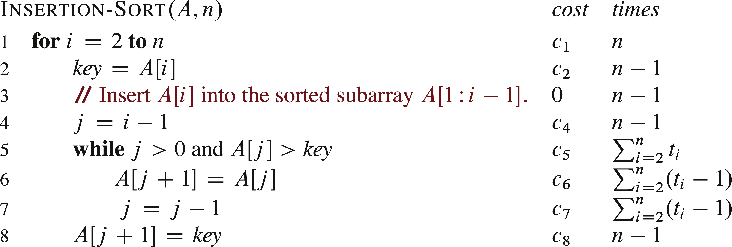
\includegraphics[angle=0]{Figures/insertion-sort-with-costs.pdf}
    \caption{Pseudocode of insertion sort with the cost of each step.}
    \label{Figure: insertion sort with costs}
\end{figure}
The running time is the cost multiplied by the number of times this step occurs. Thus the running time
for insertion sort is $T(n) = c_1 + c_2(n - 1) + c_4(n - 1) + c_5\sum_{i = 2}^{n}t_i + c_6\sum_{i = 2}^{n}(t_i - 1)
+ c_7\sum_{i = 2}^{n}(t_i - 1) + c_8(n - 1)$. Note that, while defining $t_i$ in this way simplifies the function, we could have defined it in a different
way if that were more useful.

In the best case scenario, the array was already sorted, so each \textbf{while} loop is only executed
once. That is, $t_i = 1$ (for all i) so $T(n) = (c_1 + c_2 + c_4 + c_5 + c_8)n - (c_2 + c_4 + c_5 + c_8) = an + b$, for
some constants $a$ and $b$. This is a \textit{linear} function of n.

In the worst case scenario, the array is in reverse sorted order initially. In this case, $t_i = i$ as \texttt{A[j] > key} is
true every time. We can prove the following relations by induction.
\begin{eqnarray*}
    \sum_{i = 2}^{n}i = \left(\sum_{i = 1}^{n}i\right) - 1 = \frac{n(n + 1)}{2} - 1\\
    \sum_{i = 2}^{n}(i - 1) = \left(\sum_{i = 1}^{n - 1}i\right) = \frac{n(n - 1)}{2}
\end{eqnarray*}

If we write out T(n) again, we get a function of the form $T(n) = an^2 + bn + c$, where $a$, $b$ and $c$ depend
on the constants $c_k$. This is a \textit{quadratic} function of n.

Generally, we concentrate on the worst-case running time as this gives us an upper bound for the running
time of our algorithm. Average-case running time can also be useful (for example, in the above case $t_i = \frac{i}{2})$,
although it's often the same as the worst-case. We are interested in rate of growth (or order of growth) of the running
time, that is, only the leading term. We write the order of growth with theta notation. For example, insertion
sort has $\Theta(n^2)$.

It is not common to consider the best-case running time, although there are reasons to do so. For example, the
best case of insertion sort is linear time (which is the fastest conceivable comparison sort time as every element needs to
be "looked at" at least once). We can use this initially to check if the array is already sorted, before applying
some other sorting algorithm if it isn't. This is no more computationally expensive than just running the
second algorithm immediately, which will have a running time that is greater than linear for the worst case.
Thus, we can get the benefit of quickly sorting the special case for practically no cost.

\subsection{Selection Sort}
We now introduce another sorting algorithm: \textit{selection sort}. This maintains the following loop
invariant: \textit{at the start of each outer for loop, the subarray A[1:i - 1] consists of the i - 1 smallest
elements in the array A[1:n], and they are in sorted order}. It starts with a left (empty) subarray and
the right subarray (which is just the array). It simply searches the right subarray for the
lowest element and exchanges it with the first element in the right subarray. It then iterates over this, considering
the left subarray to contain the former first element of the right array, thus shrinking the right array. This is made more
explicit in the pseudocode below:
\begin{lstlisting}
    SELECTION-SORT(A, n)
    for i = 1 to n - 1
        smallest = i
        for j = i + 1 to n
            if A[j] < A[smallest]
                smallest = j
        exchange A[i] with A[smallest]
\end{lstlisting}
This has average-case and worst-case running time $\Theta(n^2)$.

\subsection{Bubble Sort}
We will briefly mention another simple but inefficient (that is, $\Theta(n^2)$) sorting algorithm.
\begin{lstlisting}
    BUBBLE-SORT(A, n)
    for i = 1 to n - 1
        for j = n downto i + 1
            if A[j] < A[j - 1]
                exchange A[j] with A[j - 1]
\end{lstlisting}

\section{Merge Sort}
There are many algorithm design techniques. Insertion sort used the incremental method. We will now consider
the \textit{Divide-and-conquer method}.

Many useful algorithms are recursive in structure: to solve a given problem, they recurse (call themselves) one
or more times to handle closely related subproblems. These algorithms typically follow the divide-and-conquer method:
if the problem is small enough (as in the base case), you solve directly
without recursing. Otherwise, you perform the following steps: \textbf{divide} the problem into smaller instances
of the same problem; \textbf{conquer} the subproblems by solving recursively; \textbf{combine} the subproblem
solutions to form a solution to the original problem.

The merge sort algorithm follows divide-and-conquer closely. \textbf{Divide} the subarray to be sorted, \texttt{A[p:r]},
into two adjacent subarrays, each of half the size (approximately). Do this by computing the midpoint q of \texttt{A[p:r]}
(taking the average of p and r) and thus dividing A into subarrays \texttt{A[p:q]} and \texttt{A[q + 1:r]}. \textbf{Conquer} by sorting each of
the two subarrays recursively using merge sort. \textbf{Combine} by \textit{merging} the sorted subarrays back into a single sorted subarray, producing the sorted answer.
The base case is when the subarray is just one element (that is, when p = r).
\begin{lstlisting}[mathescape]
    MERGE(A, p, q, r)
    $n_L$ = q - p + 1     // Length of first subarray
    $n_R$ = r - q         // Length of second subarray
    let L[0:$n_L$ - 1] and R[0:$n_R$ - 1] be new arrays

    for i = 0 to $n_L$ - 1
        L[i] = A[p + i]
    for j = 0 to $n_R$ - 1
        R[j] = A[q + 1 + j]

    i = 0
    j = 0
    k = p

    while i < $n_L$ and j < $n_R$
        if L[i] <= R[j]
            A[k] = L[i]
            i = i + 1
        else
            A[k] = R[j]
            j = j + 1
        k = k + 1

    // Copy remainder of unmerged array accross
    while i < $n_L$
        A[k] = L[i]
        i = i + 1
        k = k + 1
    while j < $n_R$
        A[k] = R[j]
        j = j + 1
        k = k + 1
\end{lstlisting}

It may be easier to visualise this as two sorted piles of cards face up (that is so only 2 cards are visible at a time) with an empty stack face down. At each iteration,
take the visible card with the lowest value and place it face down of the initially empty pile. Iterate until one of the face up piles is empty.
At this point, flip the remaining pile and add it to the end of the facedown stack. Note that, as both piles are sorted,
the best case takes n / 2 steps as it is necessary to individually copy every card in at least one of the
piles. The worst case is n - 1 (that is, going through every card). Thus merging takes $\Theta(n)$ time. To see this,
observe that the variable initializations take constant time, the for loops take $\Theta(n_L + n_R) = \Theta(n)$
and the outcome of all the while loops is to copy every element in the array across once. Thus, the running time is $\Theta(n)$.

\begin{lstlisting}[mathescape]
    MERGE-SORT(A, p, r)
    if p >= r       // zero or one elements
        return
    q = $\lfloor$(q + r) / 2$\rfloor$
    MERGE-SORT(A, p, q)
    MERGE-SORT(A, q + 1, r)
    MERGE(A, p, q, r)
\end{lstlisting}
Note that $\lceil x \rceil$ denotes the least integer that is greater than or equal to x, and $\lfloor x \rfloor$
denotes the greatest integer that is less than or equal to x.

As an aside, \textit{coarsening} the leaves of the recursion and using insertion sort for subproblems of
a specific (and sufficiently small size) can sometimes produce a faster running time. This splits the array into $\frac{n}{k}$
subarrays of size $k$ (instead of splitting the array into $n$ subarrays of size $1$ as in traditional merge sort) and sorts each
subarray with insertion sort, then merging them as normal. This modified algorithm has running time $\Theta(nk + n\lg(n/k))$.

\subsection{Analysis of Divide-and-Conquer Algorithms}
When an algorithm contains a recursive call, you can often describe its running time by a \textit{recurrence equation}, which
describes the overall running time on a problem of size n, in terms of the running time of the same algorithm with smaller inputs.

Generally, let the worst case running time of a divide-and-conquer algorithm be given by
\[ T(n) =
  \begin{cases}
    \Theta(n)       & \quad \text{if } n < n_0\\
    D(n) + aT(\frac{n}{b}) + C(n)  & \quad \text{otherwise}
  \end{cases}
\]
where $D(n)$ is the cost to divide and $C(n)$ is the cost to combine, and the problem is divided into
$a$ subproblems of size $\frac{n}{b}$. For example, merge sort divides into two subproblmens of size
$\left \lfloor \frac{n}{2} \right \rfloor$ and $\left \lceil \frac{n}{2} \right \rceil$ respectively.

For merge sort, the divide step computes the middle of the subarray, which is constant time. The conquer step recursively
solves two subproblems of size $\frac{n}{2}$ so contributes a $2T(\frac{n}{2})$ term. Combine is executed by merge, which
we showed takes linear time. Thus $T(n) = 2T(\frac{n}{2}) + \Theta(n)$, which we can also write as
\[ T(n) =
  \begin{cases}
    c_1       & \quad \text{if } n = 1\\
    2T(\frac{n}{2}) + c_2n  & \quad \text{if } n > 1
  \end{cases}
\]
It turns out that $T(n) = \Theta(n\lg n)$, which we shall prove later. This can be intuitively seen from a recursion tree (see Figure \ref{Figure: recursion tree}).
\begin{figure}[ht]\centering
    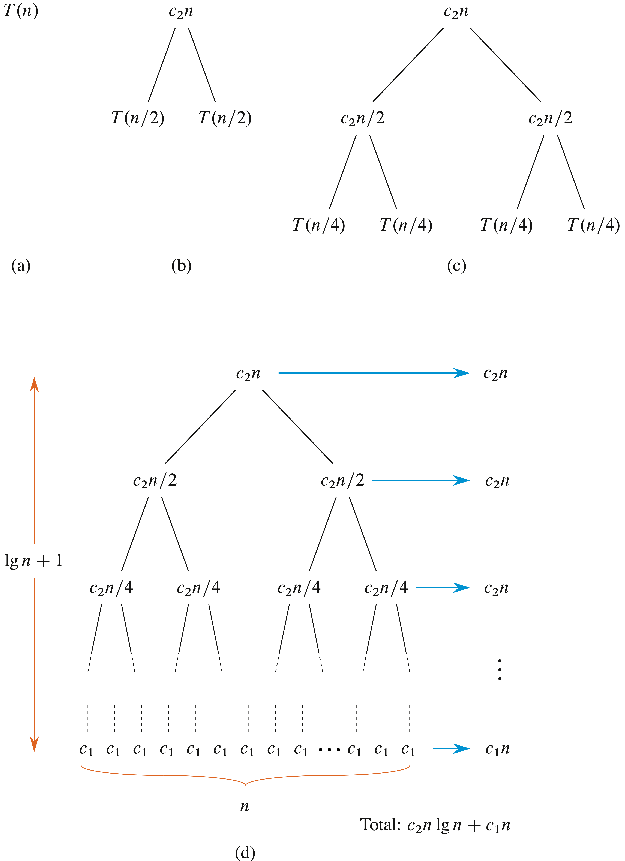
\includegraphics[angle=0]{Figures/recursion-tree.pdf}
    \caption{Recursion tree providing intuition for the total cost, by progressively expanding T(n) until
    it reaches the base case layer (the leaves).}
    \label{Figure: recursion tree}
\end{figure}

\subsection{Binary Search}
Another example of a divide-and-conquer algorithm is \textit{binary search}, which is a searching algorithm.
It specifically searches for some element $x$ in a sorted array $A$. It does this by finding the midpoint of the
boundaries of the array being searched and compares the value in this position to $x$. If they are equal, it returns
the midpoint (specifically, the index). If $x > A[mid]$, it performs the same action on the right (higher) half of the array.
Otherwise, it performs the same action on the left (lower) half of the array. This can be done iteratively (by using a while loop
that checks if the boundaries have crossed each other and updating the boundaries after each iteration) or recursively (by calling binary
search on progressively smaller subarrays). After each iteration, the number of elements to be checked halves, so binary search has a
recurrence $T(n) = T(\frac{n}{2}) + \Theta(1)$. Thus, the worst-case running time is $\Theta(\lg n)$, as this solves the recurrence.
\begin{lstlisting}[mathescape]
    RECURSIVE-BINARY-SEARCH(A, x, low, high)
    if low > high
        return NIL
    mid = $\lfloor$(low + high) / 2$\rfloor$
    if x == A[mid]
        return mid
    else if x > A[mid]
        return RECURSIVE-BINARY-SEARCH(A, x, mid + 1, high)
    else
        return RECURSIVE-BINARY-SEARCH(A, x, low, mid - 1)
\end{lstlisting}

\section{Complexity and O-notation}
When we look at input sizes sufficiently latge such that the order of growth is the only thing that impacts
the running time, we are studying the \textit{asymptotic} efficiency of algorithms. That is, how does the
running time of an algorithm depend on the size of the input $n$ in the limit $n \rightarrow \infty$.

\subsection{Asymptotic Notation}
\textbf{O-notation}: upper bound on the asymptotic behaviour of a function. That is, the function grows
no faster than a certain rate (based on the highest order term).
\newline \textbf{$\Omega$-notation}: lower bound on the asymptotic behaviour of a function. That is, the function grows
at least as fast as a certain rate (based on the highest order term).
\newline \textbf{$\Theta$-notation}: tight bound on the asymptotic behaviour of a function. That is, the function grows
precisely at a certain rate (based on the highest order term).

Note that saying the worst case running time is $\Omega(n^2)$ is not the same as saying that all inputs take
at least $cn^2$ steps, but rather that there exists at least one input, of size $n$, that takes at least $cn^2$
for every input size $n$ above a certain value.

For example, insertion sort has $O(n^2)$ as the outer \textbf{for} loop undergoes $n - 1$ iterations and the worst
case for the inner \textbf{while} loop is for it to iterate $i - 1$ times (with $i = n$ as it is the worst case). Thus, the
running time is characterised by $(n - 1)(n - 1) = O(n^2)$. It also has $\Omega(n^2)$ by the following argument: assume that
the input array has size $n$ and that the first $\alpha n$ values are the largest, where $0 < \alpha \leq \frac{1}{2}$. To sort
by insertion sort, these $\alpha n$ values need to be moved through the middle $(1 - 2\alpha)n$ positions, one position at a time,
to end up in the last $\alpha n$ positions. Thus, there are at least $\alpha(1 - 2\alpha)n^2 = \Omega(n^2)$ steps\footnote{As an aside,
this value is maximised when $\alpha = \frac{1}{4}$}. Given that the lower and upper bounds both constrain insertion sort to
quadratic time, we can also say that it has a running time of $\Theta(n^2)$.

We shall now introduce more formal definitions for asymptotic notation, which will enable us to prove various
useful relations.
\begin{definition}
    For a given function $g(n)$, we denote by $O(g(n))$ the set of functions
    \begin{multline*}
        O(g(n)) = \{f(n): \textnormal{there exist positive constants } c \textnormal{ and } n_0 \textnormal{ such that}\\
        0 \leq f(n) \leq cg(n) \textnormal{ for all } n \geq n_0\}
    \end{multline*}
\end{definition}
This definition requires that every function $f(n)$ in the set $O(g(n))$ be \textit{asymtotically nonnegative},
that is, nonnegative when $n$ is sufficiently large ($n \geq n_0$). As a result, $g(n)$ must also be asymptotically
nonnegative else the set would be empty.

\begin{definition}
    For a given function $g(n)$, we denote by $\Omega(g(n))$ the set of functions
    \begin{multline*}
        \Omega(g(n)) = \{f(n): \textnormal{there exist positive constants } c \textnormal{ and } n_0 \textnormal{ such that}\\
        0 \leq cg(n) \leq f(n) \textnormal{ for all } n \geq n_0\}
    \end{multline*}
\end{definition}

\begin{definition}
    For a given function $g(n)$, we denote by $\Theta(g(n))$ the set of functions
    \begin{multline*}
        \Theta(g(n)) = \{f(n): \textnormal{there exist positive constants } c_1, c_2 \textnormal{ and } n_0 \textnormal{ such that}\\
        0 \leq c_1g(n) \leq f(n) \leq c_2g(n) \textnormal{ for all } n \geq n_0\}
    \end{multline*}
\end{definition}
These definitions can be trivially extended to functions of multiple variables.

\begin{theorem}\label{Theorem: theta notation}
    For any two functions $f(n)$ and $g(n)$, we have $f(n) = \Theta(g(n))$ if and only if $f(n) = O(g(n))$
    and $f(n) = \Theta(g(n))$.
\end{theorem}
\begin{proof}
    Let $f(n) = O(g(n))$ and $f(n) = \Theta(g(n))$. Then, there exists a positive $c_1$ and $n_1$ such that for all $n \geq n_1$,
    $0 \leq c_1g(n) \leq f(n)$. Also, there exists a positive $c_2$ and $n_2$ such that for all $n \geq n_2$,
    $0 \leq f(n) \leq c_2g(n)$. Thus, for $n_0 = \text{max}\{n_1, n_2\}$, there exists positive $c_1$ and $c_2$ such that
    $0 \leq c_1g(n) \leq f(n) \leq c_2g(n)$ for all $n \geq n_0$. This is $f(n) = \Theta(g(n))$ by definition.

    If $f(n) = \Theta(g(n))$, then there exists positive $c_1$ and $c_2$ such that
    $0 \leq c_1g(n) \leq f(n) \leq c_2g(n)$ for all $n \geq n_0$. Clearly we can split this apart to the following
    statements: there exists a positive $c_1$ and $n_0$ such that for all $n \geq n_0$,
    $0 \leq c_1g(n) \leq f(n)$. Also, there exists a positive $c_2$ and $n_0$ such that for all $n \geq n_0$,
    $0 \leq f(n) \leq c_2g(n)$. The first statement implies that $f(n) = \Omega(g(n))$ and the second statement
    implies that $f(n) = O(g(n))$.
\end{proof}

Be careful. There are many misunderstandings that can come about from these definitions. For example, one can correctly say:
insertion sort's worst-case running time is $O(n^2)$, $\Omega(n^2)$ and, due to Theorem \ref{Theorem: theta notation}, $\Theta(n^2)$. Note
that $\Theta(n^2)$ is preferred as it is the most precise. We cannot correctly say: insertion sort's running time is $\Theta(n^2)$ as
this is not true for all cases (for example, the best case has $\Theta(n)$). However, it is still true to say its running time is $O(n^2)$ or
$\Omega(n)$ as these are true in all cases.

We cannot correctly say: "An $O(n\lg(n))$ time algorithm runs faster than an $O(n^2)$ algorithm" as the $O(n^2)$ algorithm
may actually run in $\Theta(n)$ time.

Although asymptotic notation is defined in terms of sets, we say, for example, $4n^2 + 100n + 500 = O(n^2)$ rather than using
the standard $x \in S$ notation. This abuse of notation allows us to represent anonymous functions with asymptotic
notation, saving us from naming unimportant functions. If the asymptotic notation is alone on the right hand side of
an equation, the "=" sign represents belonging. Else, the asymptotic notation represents an anonymous function. For
example, $2n^2 + 2n + 1 = 2n^2 + \Theta(n)$.

Be careful when encountering the following: $\sum_{i = 1}^{n}O(i)$ is a single anonymous function and certainly
isn't the same as $O(1) + O(2) + ... + O(n)$, which doesn't have a clear meaning.

\begin{definition}
    For a given function $g(n)$, we denote by $o(g(n))$ the set of functions
    \begin{multline*}
        o(g(n)) = \{f(n): \textbf{for all }\textnormal{positive constants } c > 0 \textnormal{, there exists } n_0 > 0 \textnormal{ such that}\\
        0 \leq f(n) < cg(n) \textnormal{ for all } n \geq n_0\}
    \end{multline*}
\end{definition}

\begin{definition}
    For a given function $g(n)$, we denote by $\omega(g(n))$ the set of functions
    \begin{multline*}
        \omega(g(n)) = \{f(n): \textbf{for all }\textnormal{positive constants } c > 0 \textnormal{, there exists } n_0 > 0 \textnormal{ such that}\\
        0 \leq cg(n) < f(n) \textnormal{ for all } n \geq n_0\}
    \end{multline*}
\end{definition}
Note that these are different from the definitions of $O(g(n))$ and $\Omega(g(n))$, which only require that some constant $c$ exists that
satisfies the inequality. $o(g(n))$ and $\omega(g(n))$, on the other hand, require the inequality to hold for all constants $c > 0$. We describe
this property as being not \textit{asymptotically tight}.

The asymptotic comparisons have some standard properties\footnote{Note, it is possible to draw an analogy between $O, \Omega, \Theta, o, \omega$ and the comparison operators
$\leq, \geq, =, <, >$.}:
\newline \textbf{Transistivity}: $f(n) = \Theta(g(n)) \text{ and } g(n) = \Theta(h(n)) \text{ implies } f(n) = \Theta(h(n))$.
This property also applies to $O, \Omega, o \text{ and }\omega$.
\newline \textbf{Reflexivity}: $f(n) = \Theta(f(n))$. This also applies to $O$ and $\Omega$.
\newline \textbf{Symmetry}: $f(n) = \Theta(g(n)) \text{ if and only if } g(n) = \Theta(f(n))$. This only applies to $\Theta$.
\newline \textbf{Transpose symmetry}:
\begin{align*}
    f(n)&= O(g(n) \text{ if and only if } g(n) = \Omega(f(n)).\\
    f(n)&= O(g(n) \text{ if and only if } g(n) = \Omega(f(n)).
\end{align*}

\section{Common functions}
We shall now take a brief break from sorting algorithms and asymptotic notation to present some miscellaneous
standard definitions and results.

A function is \textit{monotonically increasing} if $m \leq n \implies f(m) \leq f(n)$.
A function is \textit{monotonically decreasing} if $m \leq n \implies f(m) \geq f(n)$.
A function is \textit{strictly increasing} if $m < n \implies f(m) < f(n)$.
A function is \textit{strictly decreasing} if $m < n \implies f(m) > f(n)$.

$n = \lfloor n\rfloor = \lceil n\rceil$ for any integer $n$, trivially. $x - 1 < \lfloor x\rfloor \leq x
\leq \lceil x\rceil < x + 1$ for all real $x$ follows immediately from the definition. The following statements are equivalent:
$-\lfloor x \rfloor = \lceil-x\rceil$ and $-\lceil x \rceil = \lfloor-x\rfloor$. Also, for any integer
$n$ and real number $x$, we have $\lfloor n + x\rfloor = n+ \lfloor x\rfloor$ and $\lceil n + x\rceil = n+ \lceil x\rceil$.

For any integer $a$ and any positive integer $n$, the value $a\mod n$ is the \textit{remainder} or
\textit{residue} of the quotient $\frac{a}{n}$. That is, $a \mod n = a - n\left\lfloor\frac{a}{n}\right\rfloor$.
If $(a\mod n) = (b\mod n)$, we write $a = b \;(\text{mod } n)$ and say that $a$ is equivalent to $b$ modulo $n$.

Given a nonnegative integer $d$, a polynomial in $n$ of degree $d$ is a function of the form $p(n) = \sum_{i = 0}^{d}a_in^i$
where the constants $a_0, a_1, ..., a_d$ are the coefficients of the polynomial and $a_d \neq 0$. We say that
a function $f(n)$ is \textit{polynomially bounded} if $f(n) = O(n^k)$ for some constant $k$. We say that a function $f(n)$
is \textit{polylogarithmically bounded} if $f(n) = O(\lg^kn)$ for some constant k.

We can relate the growth of polynomials and exponentials with the following: for all real constants $a > 1$ and $b$, we have
$\displaystyle \lim_{n\to\infty}\frac{n^b}{a^n} = 0$, from which we can conclude that $n^b = o(a^n)$
(as $\displaystyle\lim_{n\to\infty}\frac{f(n)}{g(n)} = 0$ is a weaker definition of $f(n) = o(g(n))$).

The following results are often useful in proofs: $a^{mn} = (a^m)^n = (a^n)^m$ and $a = b^{\log_{b}a}$.

\textit{Stirling's approximation} states that $n! = \sqrt{2\pi n}\left(\frac{n}{e}\right)^n(1 + \Theta\left(\frac{1}{n}\right))$
where $e$ is the base of the natural logarithm. This gives a lower bound (and a tighter upper bound than the
more obvious $n! \leq n^n$).

Define the \textit{Fibonacci numbers} $F_i$, for $i \geq 0$ as follows:
\[ F_i =
  \begin{cases}
    0 & \quad \text{if } i = 0\\
    1 & \quad \text{if } i = 1\\
    F_{i - 1} + F_{i - 2} & \quad \text{if } i \geq 2
  \end{cases}
\]
Fibonacci numbers are related to the golden ratio $\phi$ and its conjugate $\hat{\phi}$, which are
the two roots of the equation $x^2= x + 1$, by the equation $F_i= \frac{\phi^i - \hat{\phi}^i}{\sqrt{5}}$ (which
one can prove by induction).


\end{document}
